\documentclass[]{book}
\usepackage{lmodern}
\usepackage{amssymb,amsmath}
\usepackage{ifxetex,ifluatex}
\usepackage{fixltx2e} % provides \textsubscript
\ifnum 0\ifxetex 1\fi\ifluatex 1\fi=0 % if pdftex
  \usepackage[T1]{fontenc}
  \usepackage[utf8]{inputenc}
\else % if luatex or xelatex
  \ifxetex
    \usepackage{mathspec}
  \else
    \usepackage{fontspec}
  \fi
  \defaultfontfeatures{Ligatures=TeX,Scale=MatchLowercase}
\fi
% use upquote if available, for straight quotes in verbatim environments
\IfFileExists{upquote.sty}{\usepackage{upquote}}{}
% use microtype if available
\IfFileExists{microtype.sty}{%
\usepackage{microtype}
\UseMicrotypeSet[protrusion]{basicmath} % disable protrusion for tt fonts
}{}
\usepackage[margin=1in]{geometry}
\usepackage{hyperref}
\hypersetup{unicode=true,
            pdftitle={Concepts and Computation: A Few Notes on Research Methods in Political Science},
            pdfauthor={Carlisle Rainey},
            pdfborder={0 0 0},
            breaklinks=true}
\urlstyle{same}  % don't use monospace font for urls
\usepackage{natbib}
\bibliographystyle{apalike}
\usepackage{longtable,booktabs}
\usepackage{graphicx,grffile}
\makeatletter
\def\maxwidth{\ifdim\Gin@nat@width>\linewidth\linewidth\else\Gin@nat@width\fi}
\def\maxheight{\ifdim\Gin@nat@height>\textheight\textheight\else\Gin@nat@height\fi}
\makeatother
% Scale images if necessary, so that they will not overflow the page
% margins by default, and it is still possible to overwrite the defaults
% using explicit options in \includegraphics[width, height, ...]{}
\setkeys{Gin}{width=\maxwidth,height=\maxheight,keepaspectratio}
\IfFileExists{parskip.sty}{%
\usepackage{parskip}
}{% else
\setlength{\parindent}{0pt}
\setlength{\parskip}{6pt plus 2pt minus 1pt}
}
\setlength{\emergencystretch}{3em}  % prevent overfull lines
\providecommand{\tightlist}{%
  \setlength{\itemsep}{0pt}\setlength{\parskip}{0pt}}
\setcounter{secnumdepth}{5}
% Redefines (sub)paragraphs to behave more like sections
\ifx\paragraph\undefined\else
\let\oldparagraph\paragraph
\renewcommand{\paragraph}[1]{\oldparagraph{#1}\mbox{}}
\fi
\ifx\subparagraph\undefined\else
\let\oldsubparagraph\subparagraph
\renewcommand{\subparagraph}[1]{\oldsubparagraph{#1}\mbox{}}
\fi

%%% Use protect on footnotes to avoid problems with footnotes in titles
\let\rmarkdownfootnote\footnote%
\def\footnote{\protect\rmarkdownfootnote}

%%% Change title format to be more compact
\usepackage{titling}

% Create subtitle command for use in maketitle
\newcommand{\subtitle}[1]{
  \posttitle{
    \begin{center}\large#1\end{center}
    }
}

\setlength{\droptitle}{-2em}
  \title{Concepts and Computation: A Few Notes on Research Methods in Political
Science}
  \pretitle{\vspace{\droptitle}\centering\huge}
  \posttitle{\par}
  \author{Carlisle Rainey}
  \preauthor{\centering\large\emph}
  \postauthor{\par}
  \predate{\centering\large\emph}
  \postdate{\par}
  \date{2017-12-26}

\usepackage{booktabs}

\usepackage{amsthm}
\newtheorem{theorem}{Theorem}[chapter]
\newtheorem{lemma}{Lemma}[chapter]
\theoremstyle{definition}
\newtheorem{definition}{Definition}[chapter]
\newtheorem{corollary}{Corollary}[chapter]
\newtheorem{proposition}{Proposition}[chapter]
\theoremstyle{definition}
\newtheorem{example}{Example}[chapter]
\theoremstyle{definition}
\newtheorem{exercise}{Exercise}[chapter]
\theoremstyle{remark}
\newtheorem*{remark}{Remark}
\newtheorem*{solution}{Solution}
\begin{document}
\maketitle

{
\setcounter{tocdepth}{1}
\tableofcontents
}
\chapter{Questions}\label{questions}

\begin{quote}
``The best scientists and explorers have the attributes of kids! They
ask questions and have a sense of wonder. They have curiosity. `Who,
what, where, why, when, and how!' They never stop asking questions, and
I never stop asking questions, just like a five year old.'' ---Sylvia
Earle, marine biologist
\end{quote}

See also a relevant xkcd \href{https://xkcd.com/242/}{comic}.

In political science, we ask a lot of questions about politics, such as
these questions about marriage equality:

\begin{itemize}
\tightlist
\item
  Should gay and lesbian couples have the same right to marry as
  heterosexual couples?
\item
  What percent of the public supports marriage equality for gays and
  lesbians?
\item
  What explains the recent increase in support for marriage equality?
\end{itemize}

Or these questions about income inequality:

\begin{itemize}
\tightlist
\item
  Should the government redistribute wealth?
\item
  Is income inequality higher or lower in the U.S. than France?
\item
  What are the consequences of income inequality?
\end{itemize}

In answering these questions, we might make \emph{claims} about
politics. Claims are just answers to questions. We might make the
following claims about marriage equality:

\begin{itemize}
\tightlist
\item
  Gay and lesbian couples should have the same right to marry as
  heterosexual couples.
\item
  54\% of the public supports marriage equality.
\item
  Court decisions explain the recent increase in support for marriage
  equality.
\end{itemize}

Or we might make these claims about income inequality:

\begin{itemize}
\tightlist
\item
  The government should not redistribute wealth.
\item
  Income inequality is higher in the U.S. than France.
\item
  Income inequality causes a slower growth rate.
\end{itemize}

Political science is all about \emph{asking} and \emph{answering}
questions. But the best approach to answering a question depends on the
type of question.

I break the questions we might ask (or claims we might make) about
politics into three types: normative, descriptive, and causal. Answering
each type question requires a different approach.

\begin{longtable}[]{@{}lllll@{}}
\toprule
\begin{minipage}[b]{0.17\columnwidth}\raggedright\strut
Type\strut
\end{minipage} & \begin{minipage}[b]{0.17\columnwidth}\raggedright\strut
Description\strut
\end{minipage} & \begin{minipage}[b]{0.14\columnwidth}\raggedright\strut
Marriage Example\strut
\end{minipage} & \begin{minipage}[b]{0.21\columnwidth}\raggedright\strut
Inequality Example\strut
\end{minipage} & \begin{minipage}[b]{0.12\columnwidth}\raggedright\strut
Approach\strut
\end{minipage}\tabularnewline
\midrule
\endhead
\begin{minipage}[t]{0.17\columnwidth}\raggedright\strut
normative\strut
\end{minipage} & \begin{minipage}[t]{0.17\columnwidth}\raggedright\strut
How \emph{should} the world look? Asks for a moral judgement.\strut
\end{minipage} & \begin{minipage}[t]{0.14\columnwidth}\raggedright\strut
Should gay and lesbian couples have the same right to marry as
heterosexual couples?\strut
\end{minipage} & \begin{minipage}[t]{0.21\columnwidth}\raggedright\strut
Should the government redistribute wealth?\strut
\end{minipage} & \begin{minipage}[t]{0.12\columnwidth}\raggedright\strut
logic and reasoning\strut
\end{minipage}\tabularnewline
\begin{minipage}[t]{0.17\columnwidth}\raggedright\strut
descriptive\strut
\end{minipage} & \begin{minipage}[t]{0.17\columnwidth}\raggedright\strut
How \emph{does} the world look? Asks for an empirical observation.\strut
\end{minipage} & \begin{minipage}[t]{0.14\columnwidth}\raggedright\strut
What percent of the public supports marriage equality for gays and
lesbians?\strut
\end{minipage} & \begin{minipage}[t]{0.21\columnwidth}\raggedright\strut
Is income inequality higher or lower in the U.S. than France?\strut
\end{minipage} & \begin{minipage}[t]{0.12\columnwidth}\raggedright\strut
observation and measurement\strut
\end{minipage}\tabularnewline
\begin{minipage}[t]{0.17\columnwidth}\raggedright\strut
causal\strut
\end{minipage} & \begin{minipage}[t]{0.17\columnwidth}\raggedright\strut
\emph{Why} does the world look the way it does? What \emph{influences}
X? Asks for a \emph{cause}-and-\emph{effect} relationship or an
\emph{explanation}.\strut
\end{minipage} & \begin{minipage}[t]{0.14\columnwidth}\raggedright\strut
What explains the recent increase in support for marriage
equality?\strut
\end{minipage} & \begin{minipage}[t]{0.21\columnwidth}\raggedright\strut
What are the consequences of income inequality?\strut
\end{minipage} & \begin{minipage}[t]{0.12\columnwidth}\raggedright\strut
observation and measurement, plus clever design\strut
\end{minipage}\tabularnewline
\bottomrule
\end{longtable}

\section{Normative Questions}\label{normative-questions}

Normative questions ask: ``What \emph{should} the world look like?''

In my experience, most people associate political science with normative
questions. When I tell people that I'm a political scientist, they tend
to ask me normative questions.

\begin{enumerate}
\def\labelenumi{\arabic{enumi}.}
\tightlist
\item
  ``You don't think we should invade Iran, do you?'' (Asking for a moral
  judgement about foreign policy.)
\item
  ``What do you think about the breakdown of the family in the U.S?''
  (Implicitly asking for a moral judgement about social policy, i.e.,
  ``Shouldn't the government adopt more pro-family policies?'')
\item
  ``Don't you think we're rewarding laziness?'' (Implicitly asking for a
  moral judgement about economic policy, i.e., ``We shouldn't be doing
  that, should we?''.)
\end{enumerate}

These are normative questions, if perhaps somewhat ill-formed. They are
important questions. Some political scientists, called ``political
philosophers'' or ``normative political theorists,'' focus on these
types of questions.

Some important questions asked by normative political theorists include:

\begin{enumerate}
\def\labelenumi{\arabic{enumi}.}
\tightlist
\item
  Should the state redistribute wealth?
\item
  Under what conditions is war justified?
\item
  What types of behavior should the state regulate?
\item
  How should states make policy?
\end{enumerate}

We will not focus on these types of questions.

However, we all bring normative views with us, and these views are
helpful. Normative views can motivate us to focus on certain descriptive
and causal questions. For example, perhaps you believe that democracy is
the most normatively desirable form of government. This might lead you
to describe how well democracy works in the U.S. (descriptive) or
explain why some countries remain authoritarian (causal). Perhaps you
believe that governments should not torture. This might lead you to
describe the extent to which certain states use torture (descriptive) or
the types of institutional arrangements (independent courts?) that
reduce torture (causal).

Reversing the cycle, answers to descriptive and causal questions might
inform our normative views. For example, if you know that a majority of
the U.S. public supports marriage equality, then you might think the
U.S. should allow gays and lesbians to marry. If you know that income
equality reduces economic growth, then perhaps you think the U.S. should
adopt a more redistributive economic policy.

Normative questions can motivate descriptive and causal questions.
Descriptive and causal questions can inform normative debates. But it is
important to draw a sharp distinction between normative questions and
descriptive/causal questions, because the two require completely
different approaches.

For this class, we'll not focus at all on normative questions. Instead,
we'll focus on descriptive and causal questions.

\section{Descriptive Questions}\label{descriptive-questions}

Descriptive questions ask: ``What \emph{does} the world look like?''

Descriptive questions ask for simple observations---a description of the
world.

For example, we might want to ask the following questions:

\begin{enumerate}
\def\labelenumi{\arabic{enumi}.}
\tightlist
\item
  How many chambers does the Swedish legislature have?
\item
  What percent of voters voted for Barack Obama in 2008?
\item
  How many political parties are there in the United Kingdom?
\item
  What percent of countries today are democracies? How has this changed
  over time?
\item
  What percent of eligible voters actually voted in the U.S. in 2010?
  How does this compare with turnout in other countries?
\item
  What percent of states allow same-sex marriage?
\item
  How polarized is the U.S. Congress? How has this changed over time?
\end{enumerate}

Answering these questions requires some sort of conceptualization (i.e.,
what do we mean by ``polarized''?) and measurement (i.e., how can we
quantify ``polarization''?). But all that is required is observation.
All we need to do make the appropriate measurements (i.e., gather data).

\section{Causal Questions}\label{causal-questions}

Causal questions ask: ``\emph{Why} does the work look the way it does?''

Causal questions ask about a cause or an effect. They ask for an
explanation--\emph{why} did something happen? We might be interested in
the following causal questions:

\begin{enumerate}
\def\labelenumi{\arabic{enumi}.}
\tightlist
\item
  Why is income inequality so high in the U.S.? Why is it growing so
  fast at the moment?
\item
  What causes war between two countries?
\item
  Why do some states become democratic while others remain
  authoritarian?
\item
  What is the effect of an independent court of last resort?
\item
  What explains low turnout in the U.S.?
\item
  Why do some countries have many political parties and other countries
  have few?
\item
  Why does policy change rapidly in some times and/or places, but slowly
  in others?
\item
  Does presidentialism cause democratic failure?
\end{enumerate}

Causal questions and claims are about action. We have one variable
acting on another. There are lots of verbs that summarize action:
causes, influences, affects, changes, increases, decreases, etc. Causal
questions ask us to use these sorts of verbs to describe the way the
world works.

\subsection{Meaning}\label{meaning}

We use the word ``cause'' quite a bit in everyday language. We might
say, for example, that smoking \emph{causes} cancer. In making causal
claims about politics, we might say things like ``wealth \emph{causes}
democracy'' or ``education \emph{causes} turnout.''

But what do these causal claims really mean? What does it mean for
something to \emph{cause} something else?

The idea of causation relies on the counterfactual. The counterfactual
requires us to imagine a world that does not exist (i.e., runs counter
to fact).

For example, suppose Amy has a college degree and voted in 2012. But we
want to know if the college degree caused Amy to vote. In order to
answer that question, we simply need to consider the counterfactual
world in which Amy did not receive a college degree.

We might imagine rewinding time and simply removing Amy's opportunity to
attend college (but nothing else), then letting time move forward to
2012 and observing whether Amy votes. If Amy does not vote in the
counterfactual world, then we say that the college degree caused Amy to
vote. If Amy does vote in the counterfactual world, then we say that the
college degree did not cause Amy to vote.

\begin{figure}
\centering
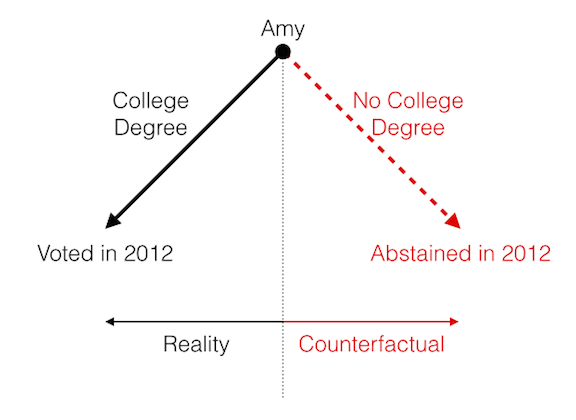
\includegraphics{diagrams/cf-amy.png}
\caption{Effect of education on turning out to vote.}
\end{figure}

\chapter{Models}\label{models}

\section{The Scientific Method}\label{the-scientific-method}

Most of us learned the scientific method as a rote process, something
like the following:

\begin{itemize}
\tightlist
\item
  Question
\item
  Hypothesis
\item
  Experiment
\item
  Analysis
\item
  Conclusion
\end{itemize}

But I don't think that's how any science, especially social science,
really works. Science is imaginative. It's creative. It's much more like
abstract painting or song-writing or poetry than replacing books in the
library (the coldest, most mechanical task I can think of).

So if science isn't rote hypothesizing and experimenting, what is it?

Let's look at Albert Einstein. Here are some things he said about his
approach to science:

\begin{quote}
When I examine myself and my methods of thought, I come close to the
conclusion that the gift of imagination has meant more to me than any
talent for absorbing absolute knowledge.
\end{quote}

\begin{quote}
All great achievements of science must start from intuitive knowledge. I
believe in intuition and inspiration\ldots{}. At times I feel certain I
am right while not knowing the reason.
\end{quote}

\begin{quote}
Imagination is more important than knowledge.
\end{quote}

\begin{quote}
I have no special talent. I am only passionately curious.
\end{quote}

In a 1961, the influential political scientist wrote the following:

\begin{quote}
\ldots{}I should like to suggest that empirical political science had
better find a place for speculation. It is a grave though easy error for
students of politics impressed by the achievements of the natural
sciences to imitate all of their methods save the most critical one: the
use of the imagination\ldots{} surely it is imagination that has
generally marked the intelligence of the great scientist, and
speculation---often-times foolish speculation, it turned out later--has
generally preceded great advances in scientific theory.
\end{quote}

The scientific method is (sometimes serendipitous) interaction between
speculation and observation.

\begin{figure}
\centering
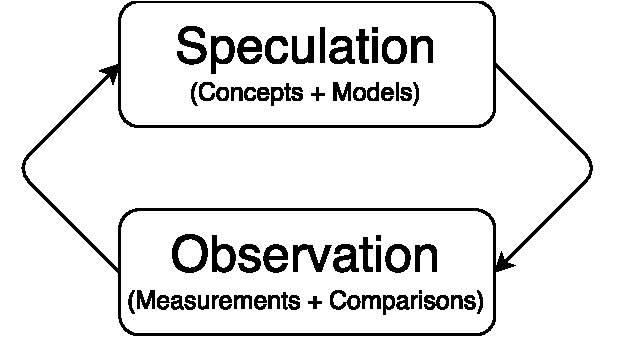
\includegraphics{diagrams/speculation-observation.pdf}
\caption{A figure illustrating the relationship importance of
speculation and imagination in science.}
\end{figure}

My version of the scientific method is

\begin{itemize}
\tightlist
\item
  Concepts
\item
  Models
\item
  Measurements
\item
  Comparisons
\end{itemize}

The first two components, concepts and models, we might refer to as
``speculation.'' I like this term, because it emphasizing the carefree,
creative nature scientific notions. Many students are too afraid of
being wrong. ``speculation'' frees us up to use our imagination.

\subsection{Concepts}\label{concepts}

Concepts are simply mental constructs. For our purposes, concepts are
words that we use to describe political entities. For example, we can
use the concept of ``democracy'' and describe the United States as a
democracy. We can use the concept of ``liberal'' and refer to Nancy
Pelosi as a liberal.

Concepts are important because they allow us to communicate and reason
precisely and accurately about political events. In general, ambiguous
concepts need work. We need precise, well-defined concepts. They will
never be perfect, but we should always push ourselves toward more
precision and clarity.

Some concepts are easier to define precisely than others, for example.
``Vote share''" is easy to define. ``Democracy'' and ``ideology'' are
not so easy.

To illustrate, answer the following question: What is a democracy? This
is harder than it seems.

Concepts in political science tend to be more abstract and ill-defined.
But it is essential to define our concepts as precisely as possible.
Before we can answer questions about our concepts, we must know what our
concepts mean!

Does negativity cause an increase or a decrease in turnout? To answer
this, we certainly need to know if ``The incumbent voted for Obamacare''
is considered negativity.

\subsection{Models}\label{models-1}

A model is simply a tentative explanation of observed phenomena, used to
better understand the world. Models need not be accurate in every
respect. A model is sometimes referred to as a theory, explanation, or
story.

Models connect concepts in a causal fashion. One minimal model, for
example, is that increasing the level of democracy in a country leads to
more economic growth. In this case, we have two concepts, democracy and
economic growth, connected causally. Of course, we'd want to elaborate a
bit and flesh this model out into a fuller explanation. Why is it,
exactly, that democracy causes growth?

We can also think of models as logical defenses or justifications of
causal claims. For example, we might take two or three basic principles
or axioms as given, and deduce causal claims from this. For example, we
might assume that people behave in a way that benefits them most
financially. We might also assume that the Republicans tend to adopt
lower tax rates than Democrats. Therefore, it seems reasonable to
conclude that an increase in one's wealth makes them more likely to vote
Republican.

\subsection{Measurements and
Comparisons}\label{measurements-and-comparisons}

We'll spend some time later in the semester talking about measurements
and comparisons. But for now, simply note that measurements are simply
quantifications of our concepts. In order to study a phenomenon
systematically, we often want to assign numbers to the entities of
interest. If we are interested in the concept of economic growth, for
example, then the percent change in GDP is a good way to quantify that
concept. Similarly, if we are interested in democracy, then we might
develop a process for assigning each country a score from -10 to 10,
where -10 represents the least democratic countries and 10 represents
the most democratic countries.

Once we have these measures, we'll want to make the appropriate
comparisons. For example, we might want to compare the average economic
growth in democracies and non-democracies.

\section{Building Models}\label{building-models}

But how do you build a model? How do you put together a compelling
logical defense of a causal claim?

A model of the model-building process:

\begin{itemize}
\tightlist
\item
  Step 1: Observe some facts. If these facts are puzzling, even better.
  (e.g., a large percentage of people vote, countries fight
  wars---notice that our models are what make these facts puzzling)
\item
  Step 2: Look at the facts as though they were the end result of some
  unknown process (model). Then speculate about the process that might
  have produced such a result. We're thinking in terms of causation here
\item
  Step 3: Deduce other results (implications, hypotheses, or
  predictions) from the model.
\item
  Step 4: Then ask yourself whether these other implications are true
  and produce new models if necessary.
\end{itemize}

Some rules of thumb for model-building:

\begin{itemize}
\tightlist
\item
  Rule 1: Think ``process.'' In particular, think about causality. One
  thing leads to another, which causes two changes, which both affect
  the concept we care about.
\item
  Rule 2: Develop interesting implications. An interesting implication
  might be one that would otherwise (i.e., in the absence of the model)
  be counterintuitive. It might also be an implication for which we have
  the appropriate data.
\item
  Rule 3: Look for generality. If you start with a theory about US voter
  behavior, can you generalize it to voting behavior in other places?
  Finding generalizations usually involves generalizing nouns.
\item
  Rule 4: Realize that model-building is a slow process
\item
  Rule 5: Talk about your ideas.
\end{itemize}

\section{Evaluating Models}\label{evaluating-models}

Truth

\begin{itemize}
\tightlist
\item
  Are the implications of the model correct?

  \begin{itemize}
  \tightlist
  \item
    What about the assumptions? In practice, we don't worry much about
    the assumptions for a few reasons. Assumptions are usually
    simplifications (e.g., politicians are office-seeking). Many good
    models are based on simple, but incorrect assumptions.

    \begin{itemize}
    \tightlist
    \item
      Assumptions sometimes cannot be observed directly.
    \item
      Testing assumptions distracts your attention from the implications
      of the model. Get it the habit of exploring and evaluating the
      range of implications of the model.
    \item
      That said, all else equal, we would prefer a model based on
      correct assumptions.
    \end{itemize}
  \end{itemize}
\item
  In particular, the model should allow us to make predictions (note
  that we can have a predictive model, that is not necessarily causal.
  However, causal models should be predictive of future observations.)
\end{itemize}

Question: How could we evaluate the truth of our model of ACA opinions?

\begin{itemize}
\tightlist
\item
  Beware of circular or tautological models (e.g., people do what is in
  their self interest)
\item
  Find critical experiments. The ideal approach is to compare
  alternative models. When we have two competing models, we'd like to
  find a situation in which the two model produce different
  implications. This is a powerful situation, because only one of the
  models can be correct.
\item
  To the extent possible, always think in terms of alternative models,
  as opposed to a single model being right or wrong.
\end{itemize}

Beauty (e.g., Downs)

\begin{itemize}
\tightlist
\item
  Simplicity (office-seeking) - some assert that simpler models are more
  likely to be correct.
\item
  Fertility (produces many implications)
\item
  Surprise (why is turnout so high?)
\end{itemize}

Justice - does the model advance normative goals?

\section{Review Exercises}\label{review-exercises}

\begin{enumerate}
\def\labelenumi{\arabic{enumi}.}
\tightlist
\item
  Describe (my view of) the scientific method. How do concepts, models,
  measurements, and comparisons all fit together.
\item
  Summarize my model of the model-building process.
\item
  What are the five rules of thumb for model-building?
\item
  How do we evaluate models? Which of the three criteria do you feel are
  most and least important?
\item
  What is a critical test and why is it important?
\end{enumerate}

\bibliography{book.bib,packages.bib}


\end{document}
